\subsection{Información personal}

  \subsubsection{Ver información personal}

  \paragraph{}Este usuario tendrá la posibilidad de ver y editar la información
  personal que está albergada en el sistema. Esta operación se realiza mediante
  el formulario de edición de información personal, el cual se muestra en la
  figura \ref{capturaModificarDatosAsesor}.

  \begin{figure}[!ht]
    \begin{center}
      \fbox{
      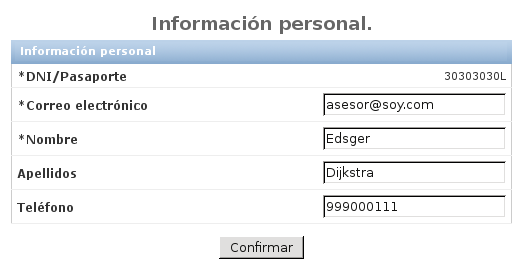
\includegraphics[scale=0.55]{4.Funcionamiento_Aplicacion/4.3.Gestion/4.3.3.Asesor/4.3.3.9.InformacionPersonal/edit_datos_asesor.png}
      }
      \caption{Captura de pantalla del formulario de edición de datos personales para el usuario \textit{Asesor}.}
      \label{capturaModificarDatosAsesor}
    \end{center}
  \end{figure}


  \subsubsection{Modificar contraseña}

  \paragraph{}Para este usuario, estará disponible la posibilidad de cambiar su
  contraseña en el sistema. Para llevar a cabo esta operación, deberá seguir los
  mismos pasos indicados en la sección \ref{modificarPassword}.

  \paragraph{}Una vez rellenado el formulario, se pulsará el botón
  \textit{Confirmar}, el cual se puede ver en la figura
  \ref{capturaBotonConfirmar}. Si el formulario rellenado es válido, y no tiene
  errores, se editará la información personal en el sistema. En caso de
  contener información no válida, un mensaje de error aparecerá indicando los
  campos del formulario que no han pasado la validación, los cuales habrá que
  modificar para modificar correctamente los datos personales en el sistema.
